\chapter{陈省身微分几何讲义}\index{陈省身微分几何讲义}
\section{流形的基本概念}\index{流形的基本概念}
\begin{thm}
\begin{enumerate}[label=(\arabic*),font=\upshape]
    \item 给定 $M,N$ 为两个 $n$维光滑流形且 $f$是从 $M$到 $N$的光滑映射.\cite{吴大任1979微分几何讲义}
    \item 在 $M$上一点 $p$处, $f$诱导的切映射 $f_*\colon T_p (M)\to T_{f(p)}(N)$是同构.
\end{enumerate}
则存在一点$p$在 $M$中的邻域 $U$, 使得 $V=f(U)$为 $f(p)$在 $N$中一邻域且 $f|_U\colon U\to V$是可微同胚.
\end{thm}
\begin{proof}
    由于 $f:M\to N$ 是光滑映射.故取 $p$在 $M$中局部坐标系 $(U_),\varphi)$和 点 $q=f(p)$在 $N$中局部坐标系 $(V_0,\psi)$,使得 $f(U_0)\subseteq V_0$,且
    \begin{eq*}
        \tilde{f}=\psi\circ f \circ \varphi^{-1}\colon \varphi (U_0)\to \psi (V_0) \subset \R^n.
    \end{eq*}
    是光滑映射.
    \begin{figure}[h]
        \begin{small}
            \begin{center}
                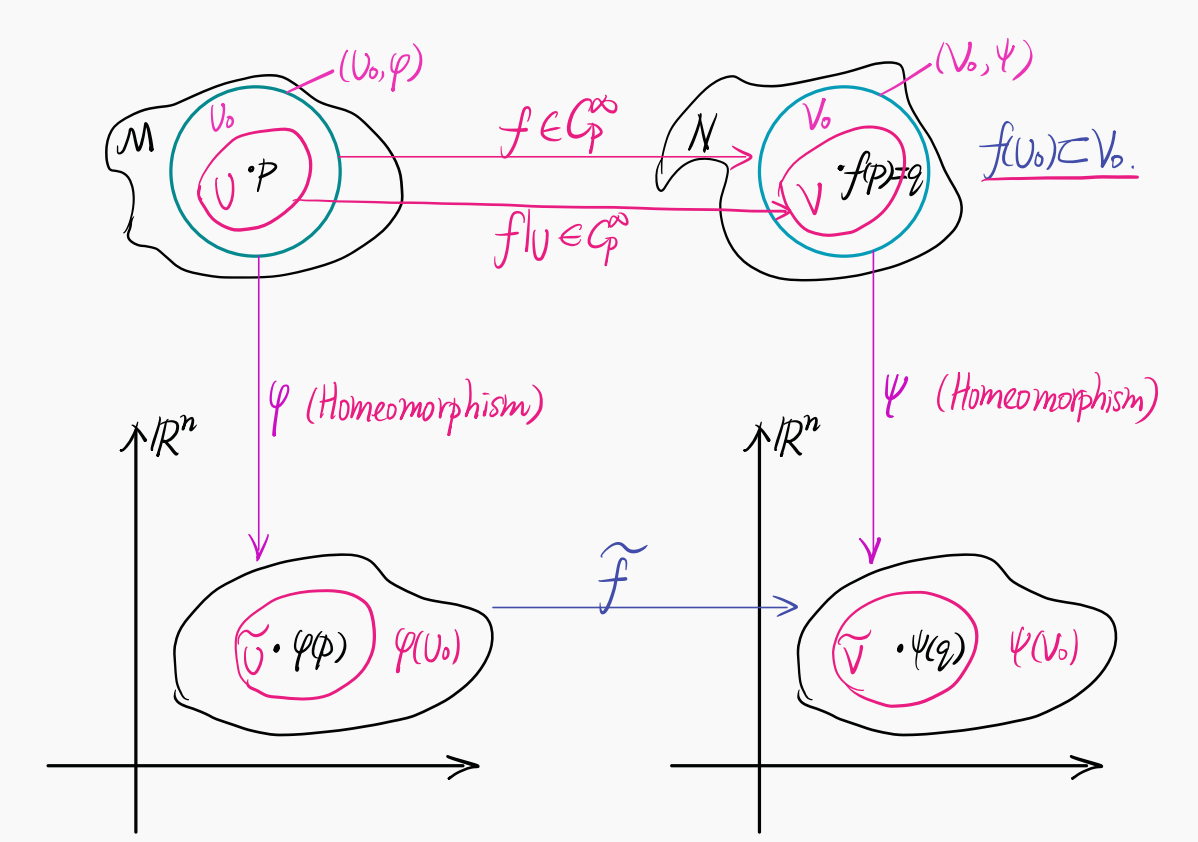
\includegraphics[width=0.6\textwidth]{figures/thm3.4.png}
            \end{center}
            \caption{图示}
            \label{fig:thm3.4proof}
        \end{small}
    \end{figure}
    
    故 $\tilde{f}=\psi\circ f\circ \varphi^{-1}$是光滑的. $\varphi(U_0)$与 $\psi(V_0)$均是 $\R^n$中的开集.在定理3.1中,令 $x_0=\varphi(p),f=\tilde{f}$,则若 $\det \left(\frac{\partial f^i}{\partial x^j}\right)\bigg|_{x_0}\neq 0$,则存在 $\varphi(p)$与$\psi(q)$在 $\varphi(U_0)$与 $\psi(V_0)$的邻域 $\widetilde{U}$与 $\widetilde{V}$,使得 $\tilde{f}|_{U_0}\colon \widetilde{U}\to\widetilde{V}$是可微同胚.

    令 $U=\varphi^{-1}(\widetilde{U}),V=\psi^{-1}(\widetilde{V})$,则 $U$与 $V$分别是$p$与 $q$在 $M$与 $N$中的邻域,且$f|_{U}=\psi^{-1}\circ \tilde{f}\circ \varphi\colon U\to V$是可微同胚.

    为何 $\tilde{f}$在 $\varphi(p)$的Jacobi行列式非零是显然的?
    由于
    \[
    \begin{aligned}
        & \left.\operatorname{det}\left(\frac{\partial f^i}{\partial x^j}\right)\right|_{x_0} \neq 0 . \Leftrightarrow f_*: T_{x_0} M\left(\simeq \mathbb{R}^n\right) \longrightarrow T_{f_{(x_0)}}\left(\mathbb{R}^n\right)\left(\simeq \mathbb{R}^n\right) \\
        & \left.\operatorname{det}\left(\frac{\partial \tilde{f}^i}{\partial x^j}\right)\right|_{\varphi(p)} \neq 0 \Leftarrow \tilde{f}_*: T_{\varphi(p)} M \left(\simeq \mathbb{R}^n\right) \longrightarrow T_{\tilde{f} \varphi(\rho)}\left(\mathbb{R}^n\right) (\simeq \mathbb{R}^n) 
        \end{aligned}\]
        故映射 $f$的 Jacobi矩阵 $\left(\frac{\partial f^i}{\partial x^j}\right)$恰是 $f_*$在自然基底下的矩阵.
\end{proof}
\subsection{小结}
\begin{itemize}
    \item 余切空间 $T^*_p =\F_p/\mathcal{H}_p=\{(\dd f)_p\}$,
    \item 自然基底 $\{(\dd u^i)_p,1\leqslant i\leqslant n\}$,
    \item 余切空间之间的光滑映射:
    \[F^*\colon T^*_q\to T^*_p\; \text{(设 $F\colon M\to N$是光滑映射且 $q=F(p)$.)}\]
    \begin{itemize}
        \item 作用方式 \quad $(\dd f)_p\mapsto \dd(f\circ F)$,
        \item 在两个自然基底下的矩阵表示: 
        
        设 $u^i$是 $p$附近的局部坐标表示, $v^\alpha$是 $q$附近的局部坐标表示,则映射 $F$在点$p$附近可用函数
        \begin{equation}
            \label{eq:valpha}
            v^\alpha=F^\alpha (u^1,\cdots,u^m),1\leqslant \alpha\leqslant n,
        \end{equation}
        表示.

        注解: \begin{eq*}
            v^\alpha &=(\psi(q))^\alpha=(\psi\circ F(p))^\alpha=(\psi\circ F\circ \varphi^{-1}(u^1,\cdots,u^m))^\alpha\\
            &\xlongequal[]{\text{令 $F^\alpha=\psi\circ F\circ \varphi^{-1}$}} F^\alpha (u^1,\cdots,u^m)
        \end{eq*}
        因此, $F^*$在自然基底 $\{\dd v^\alpha,1\leqslant\alpha\leqslant n\}$作用下结果为
        \begin{eq*}
                    F^* (\dd v^\alpha)=\dd (v^\alpha\circ F)=(\dd (F^\alpha(u^1,\cdots,u^m)))_p=\sum_{i=1}^{m}\left(\frac{\partial F^\alpha}{\partial u^i}\right)_p \cdot (\dd u^i).
        \end{eq*}
        从而 $F^* \{\dd v^\alpha\}=J\{\dd u^i\}$,其中 $J=\left(\frac{\partial F^\alpha}{\partial u^i}\right)_p$为 \eqref{eq:valpha}函数的Jacobi矩阵.
    \end{itemize}
    \item 
\end{itemize}



















